\documentclass{article}

\usepackage{amsmath}
\usepackage{amsfonts}
\usepackage{amssymb}
\usepackage{graphicx}
\usepackage[dvipsnames]{xcolor}
\usepackage[margin=0.5in]{geometry}
\usepackage[hidelinks]{hyperref}
\usepackage{enumitem}
\usepackage{changepage}
% \usepackage{rotating}

\graphicspath{{.}{./img/}}

\usepackage{environ}
\NewEnviron{centerframebox}{\begin{center}\fbox{\parbox{0.92\textwidth}{\BODY}}\end{center}}

\title{Algorithms for Data Science \\ Exercise Sheet 2}
\author{
  Vladislav Imashev \\ \href{mailto:s05vimas@uni-bonn.de}{s05vimas@uni-bonn.de} \and
  AAAAAAAAAA AAAAAAA \\ \href{mailto:AAAAAAAAAAAAAAAAAAAA}{AAAAAAAAAAAAAAAAAAAA} \and
  German Mikhelson \\ \href{mailto:s17gmikh@uni-bonn.de}{s17gmikh@uni-bonn.de} \and
  Aleksandra Volynets \\ \href{mailto:s02avoly@uni-bonn.de}{s02avoly@uni-bonn.de} \and
  Nikita Morev \\ \href{mailto:s99nmore@uni-bonn.de}{s99nmore@uni-bonn.de}
}

\begin{document}
  \maketitle

  \setcounter{section}{2}
  \subsection{DFS Listing}
  \begin{centerframebox}
    A database has the following five transactions:

    % this is the same database as last lime
    \begin{center}
      \begin{tabular}{|c|c|}
        \hline
        TID & items bought \\ \hline
        1 & M, O, N, K, E, Y \\ \hline
        2 & D, O, N, K, E, Y \\ \hline
        3 & M, A, K, E \\ \hline
        4 & M, U, C, K, Y \\ \hline
        5 & C, O, K, E \\ \hline
      \end{tabular}
    \end{center}

    List all frequent itemsets with a minimum support of $0.6$ (i.e., $t = 3$) by the
    DFS Listing algorithm. Give the details of your computation including all projected datasets computed by the algorithm.
  \end{centerframebox}
  \textit{Solution:}

  In the first step, we have to remove the values that: $count(i) \leq threshold$

  So, on the first step we remove: \textbf{A, C, D, N, U}

  Let's arrange the remaining letters in alphabetical order:
  $E < K < M < O < Y$

  Answer: \textbf{\{EO, EKY, EKMO, EKMY, EKO, EY, EMO, EMY, KY, KMO, KMY, KO, O, MO, MY\}}

  \begin{adjustwidth}{-0.5in}{-0.5in}
    \centering
    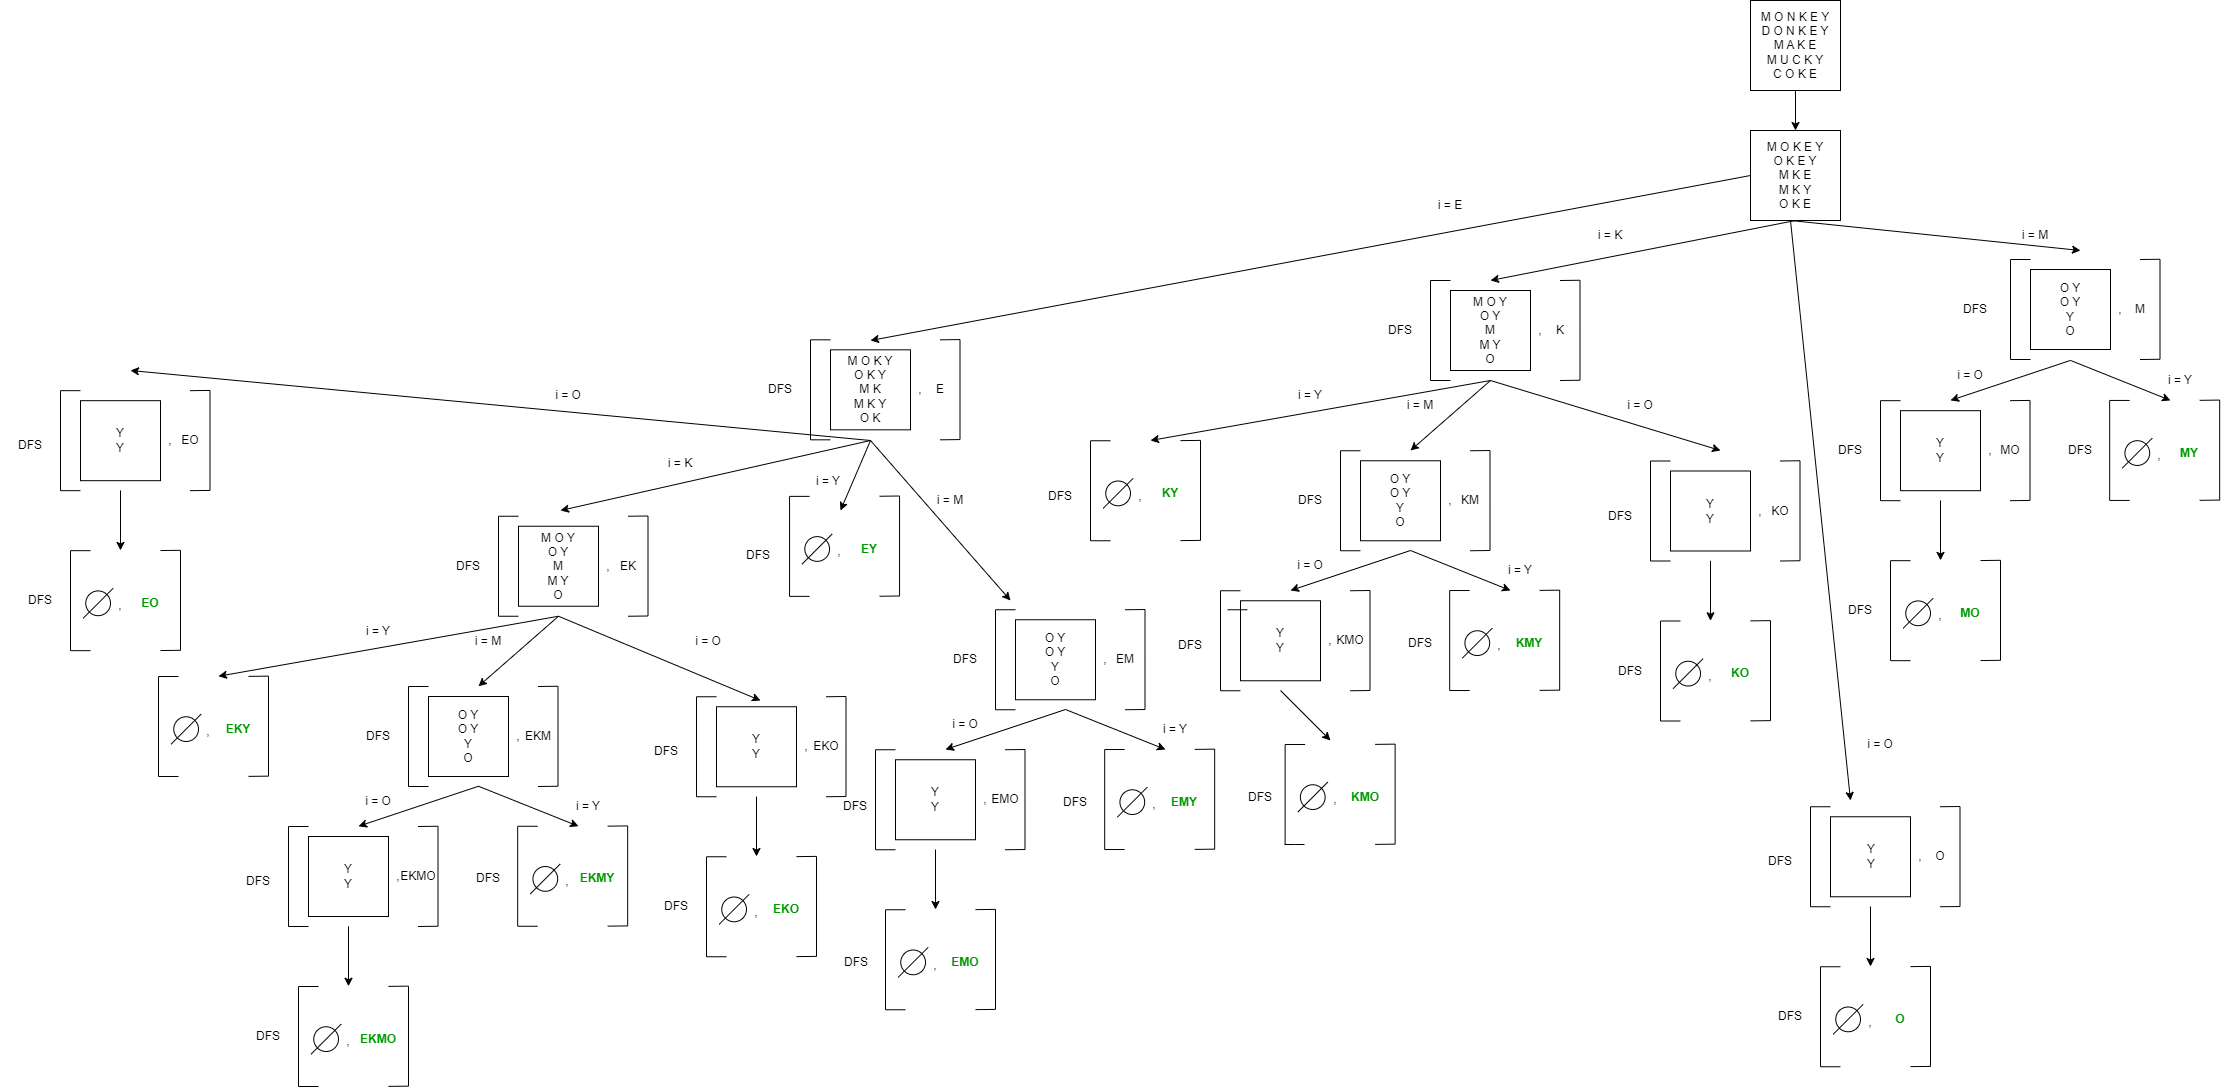
\includegraphics[width=1.13\textwidth]{Task1_DS.png}
  \end{adjustwidth}

  % \begin{sidewaysfigure}[ht]
  %   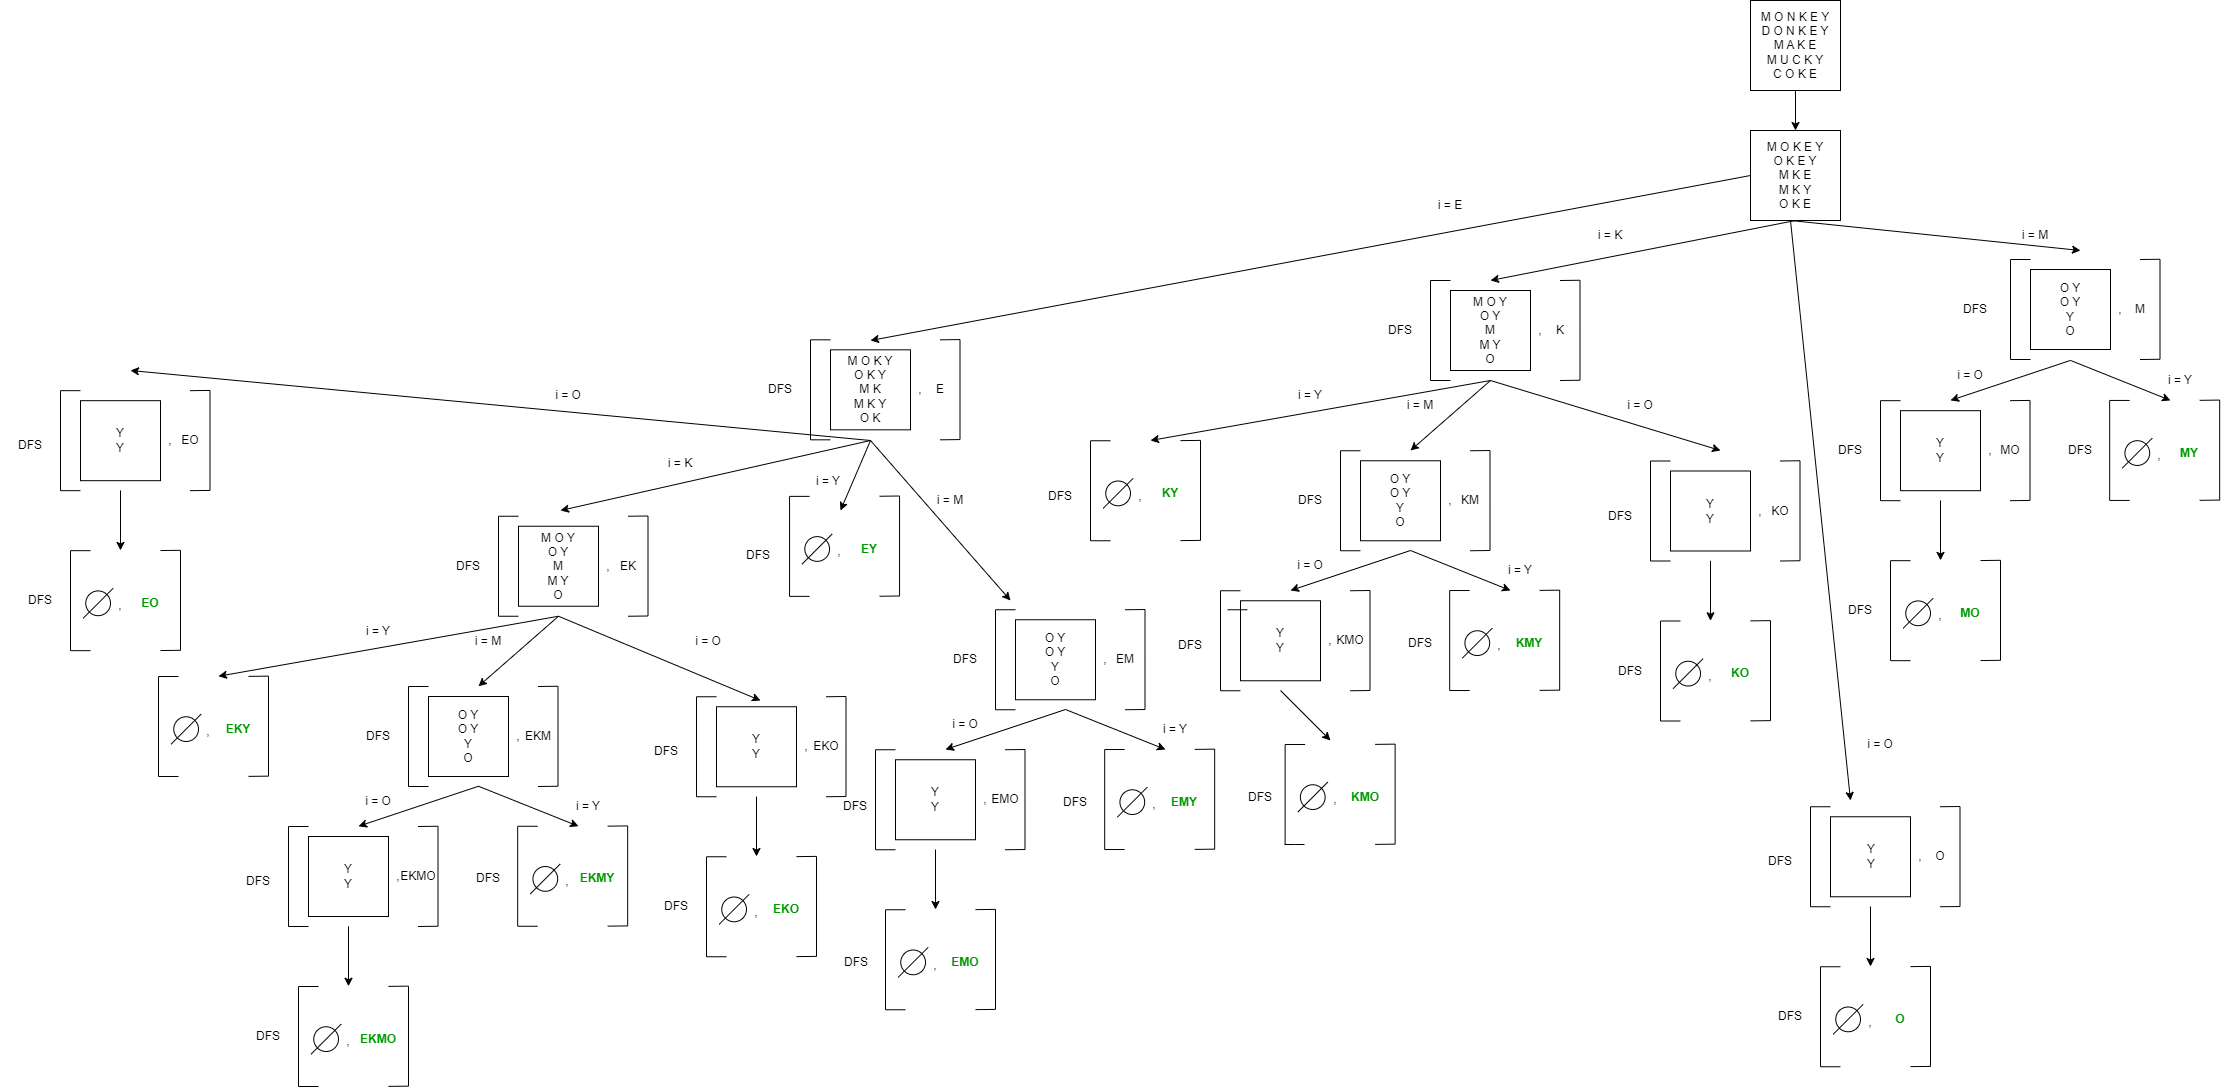
\includegraphics[width=\textwidth]{Task1_DS.png}
  %   \caption{The call tree produced by the DFS Listing algorithm.}
  %   \label{fig:LandscapeFigure}
  % \end{sidewaysfigure}

  \subsection{Properties of DFS Listing}
  \begin{centerframebox}
    Prove the proposition on Slide 7 of 2023-11-08.

    \textbf{Proposition}: the previous algorithm correctly and irredundantly enumerates all
    frequent itemsets with \textit{polynomial delay}.
    \begin{itemize}
      \item \textbf{correct}: sound and complete
      \begin{itemize}
        \item \textbf{sound}: all itemsets outputted are frequent and
        \item \textbf{complete}: all frequent itemsets are generated
      \end{itemize}
    \end{itemize}
  \end{centerframebox}
  \subsubsection*{Proving soundness}
  Can we print an infrequent item?

  No: since every call to the DFS\_Listing prompts algorithm to remove every infrequent item from given transaction database on the second step.

  \subsubsection*{Proving completeness}
  Assume there are frequent itemsets, that are not generated by our algorithm.
  Let $Z$ be inclusion minimal in these sets.

  If $Z$ is just a single element set, it would have been added in the first step.
  Let $m$ be the largest item in $Z$ (according to the total order) and $X := Z \setminus \{m\}$ be a subset of $Z$.
  By minimality of $Z$, all $(|Z| - 1)$ length subsets of $Z$ are in $F$ at some point of the algorithm.

  Let's consider a call to the DFS algorithm on $X$.
  In this step $D$ contains a projection of this subset on the database (as it was calculated in the previous call to this algorithm).
  Since $m$ is a frequent item, it doesn't get removed on the second step.
  Then, according to the for-loop we consider every item that is left in given projection $D$ and add it to $F$.
  Consequently, this means $X \cup m$ will be added to $F$ and be printed.

  \subsubsection*{Proving irredundancy}
  All single item sets are simply added to $F$ in the first step, no possibility of multiple instances.

  Let's consider two different frequent items $m$ and $n$, where $m > n$ by total order.
  An item is only added to the itemset if it is frequent in the projection of this itemset on the previously considered database.
  This projection contains only items that are larger by total order, which means projection $D_m$ doesn't contain item $n$.
  As the itemset cannot be created by any other means, so we don't generate any redundancies.

  \subsubsection*{Proving polynomial delay}
  Let's consider the algorithm between the printings of frequent items.
  Let $D_i$ be projection of given database and $I_i$ a set of items present in $D_i$.
  First every item that is present in $D_i$ is checked for frequency: $O(|I_i||D_i|)$.
  Then for every item that is left after removal of infrequent items algorithm creates a projection:
  $O(|D_i|)$ and calls for the next iteration of the algorithm.
  This call prompts the next printing of $F$.
  The time between this action and the previous printing of $F$ is bounded by:
  $O(|I_i||D_i|2)$, where $|I_i| \leq |I|$ and $|D_i| \leq |D|$ and for each call of the algorithm these values do not increase.
  If we consider the whole algorithm the time would be bounded by $O(|F||I||D|2)$.

  \subsection{FP-Tree}
  \begin{centerframebox}
    \begin{enumerate}[label=(\roman*)]
      \item Construct an FP-tree for the transaction dataset and minimum support
      given in Task 1 above.
      \item  Let the transaction database be $\mathcal{D} = \{ab,\, ac,\, bcd,\, bd,\, cd,\, d\}$ and the frequency threshold $t = 1$.
      Is the heuristic used in the FP-Tree construction algorithm (see steps 1 and 2 on Slide 10 of 2023-11-08)
      \textit{optimal} for $\mathcal{D}$ and $t$? (We want to build an FP-Tree with as few nodes as possible.)
    \end{enumerate}

    Steps 1 and 2 on Slide 10 of 2023-11-08:
    \begin{enumerate}[label=\arabic*:]
      \item compute the set $I'$ of frequent items and their support
      \item sort $I'$ in support descending order
    \end{enumerate}
  \end{centerframebox}
  \begin{enumerate}[label=(\roman*)]
  \item Frequency threshold $t = 3$, hence:
    \begin{center}
      \begin{tabular}{|c|c|}
        \hline
        TID & items bought \\ \hline
        1 & M, O, \textcolor{red}{N}, K, E, Y \\ \hline
        2 & \textcolor{red}{D}, O, \textcolor{red}{N}, K, E, Y \\ \hline
        3 & M, \textcolor{red}{A}, K, E \\ \hline
        4 & M, \textcolor{red}{U}, \textcolor{red}{C}, K, Y \\ \hline
        5 & \textcolor{red}{C}, O, K, E \\ \hline
      \end{tabular}
    \end{center}
    $$I' = \{ \text{K : } 5, \text{ E : } 4,\text{ Y : } 3,\text{ M : } 3,\text{ O : } 3 \}$$
    \begin{center}
      \begin{tabular}{|c|c|}
        \hline
        TID & items bought pruned and sorted \\ \hline
        1 & K, E, Y, M, O \\ \hline
        2 & K, E, Y, O \\ \hline
        3 & K, E, M \\ \hline
        4 & K, Y, M \\ \hline
        5 & K, E, O \\ \hline
      \end{tabular}
    \end{center}

    \begin{center}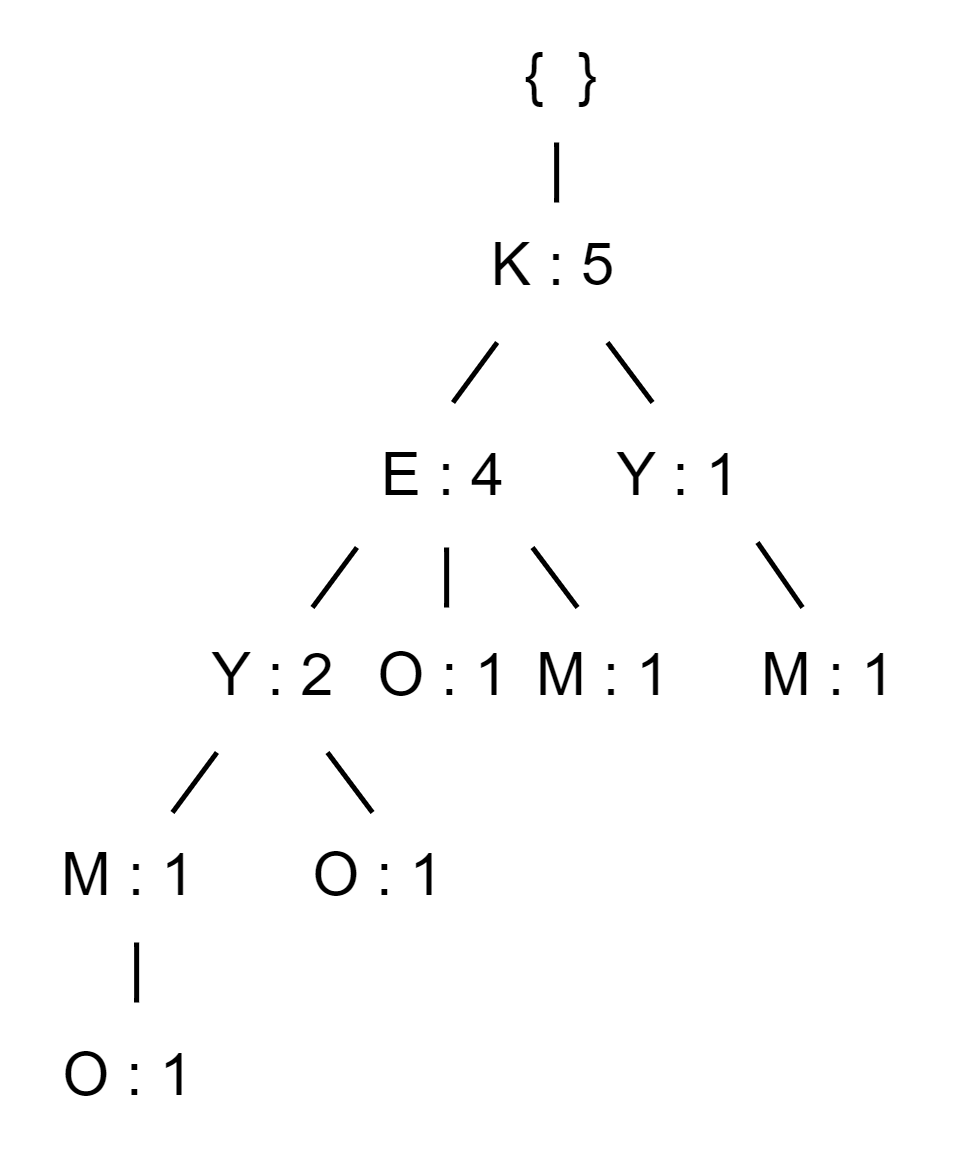
\includegraphics[scale=0.25]{Task3_DS_a.png}
    \end{center}

    \item We have the following database:
    \begin{center}
      \begin{tabular}{|c|c|}
        \hline
        TID & items \\ \hline
        1 & a, b \\ \hline
        2 & a, c \\ \hline
        3 & b, c, d \\ \hline
        4 & b, d \\ \hline
        5 & c, d \\ \hline
        6 & d \\ \hline
      \end{tabular}
    \end{center}
    Hence
    $$I' = \{ \text{d : } 4, \text{ b : } 3,\text{ c : } 3, \text{ a : } 2 \}$$
    \begin{center}
      \begin{tabular}{|c|c|}
        \hline
        TID & items sorted \\ \hline
        1 & b, a \\ \hline
        2 & c, a \\ \hline
        3 & d, b, c \\ \hline
        4 & d, b \\ \hline
        5 & d, c \\ \hline
        6 & d \\ \hline
      \end{tabular}
    \end{center}
    \begin{center}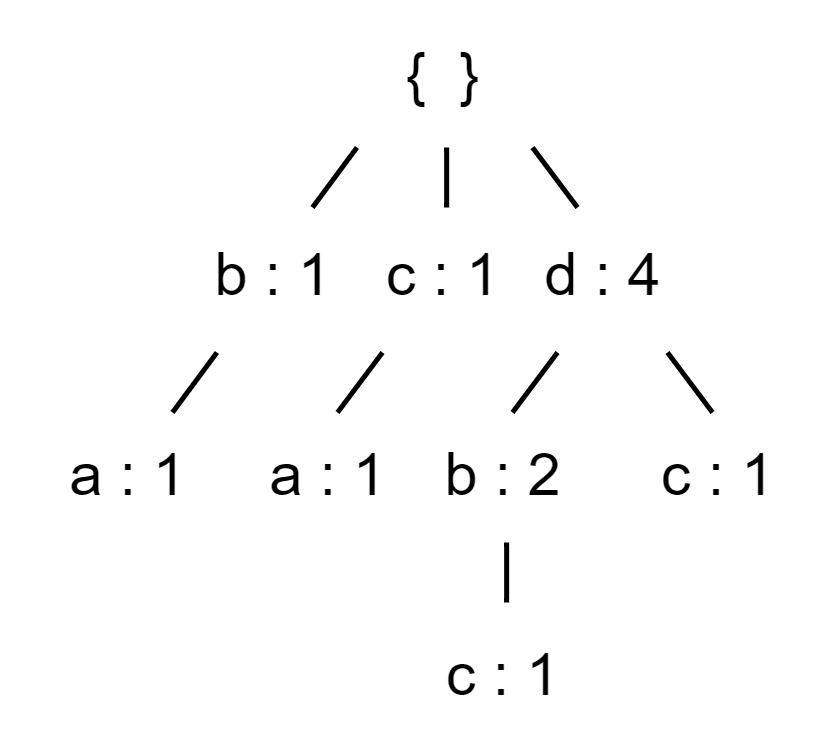
\includegraphics[scale=0.3]{Task3_DS_b.png}
    \end{center}
    Steps 1 and 2 in the algorithm help to construct smaller tree so the common parts (in particular, frequent prefixes) of the itemsets will be shared in the tree. Therefore, in the result tree we will have as few nodes as possible.
  \end{enumerate}

  \subsection{Counting Frequent Itemsets}
  \begin{centerframebox}
    Prove the claim on Slide 25 of 2023-11-08.

    \textbf{Claim}: an assignment falsifies $f$ $\iff$ the set of items corresponding to the variables with value 1 forms a frequent itemset for $t = 1$
    % $\Rightarrow$ number of satisfying assignments of $f$:
    % \[ 2^n -\textrm{ number of }1\textrm{-frequent itemsets }- 1 \]

    \[ f = (x_1 \lor x_2) \land (x_2 \lor x_3) \land (x_1 \lor x_4) \qquad\Rightarrow\qquad
      \begin{matrix}
        & x_1 & x_2 & x_3 & x_4 & x_5 \\
        x_1 \lor x_2 & 0 & 0 & 1 & 1 & 1 \\
        x_2 \lor x_3 & 1 & 0 & 0 & 1 & 1 \\
        x_1 \lor x_4 & 0 & 1 & 1 & 0 & 1 \\
      \end{matrix}
    \]
  \end{centerframebox}
  First let's prove the ``$\Leftarrow$'' direction.
  If the itemset is frequent for $t = 1$, this just means it occurs at least once.
  Every transaction in our database excludes exactly two items, because they correspond to the variables that for the corresponding clause in our 2CNF expression $f$.
  This means that the two variables present in this clause are not part of our assignment, and this clause evaluates to \texttt{false}.
  And this means that the whole $f$ formula evaluates to 0 as well, i.e. it is falsified by our assignment.

  Proving the other ``$\Rightarrow$'' direction is about the same.
  If our assignment falsifies $f$, then there exists a false clause $\exists (x_n \lor x_m) = 0$ in the our 2CNF expression $f$,
  and both variables $x_n$ and $x_m$ must be 0 in our assignment.
  The clause $(x_n \lor x_m)$ will have a correspond transaction $X \in D$ in the database,
  and this transaction will include all items except for $x_n$ and $x_m$,
  and we already know that $x_n$ and $x_m$ are false in our assignment,
  so $X$ must include all true items (items that correspond to variables, that have been assigned 1 by our assignment).
  This way the itemset of all true items will be part of $X$ and thus have a frequency greater than or equals to $t = 1$.
  $\blacksquare$

\end{document}
